% 20-minute talk (cryptographic audience) on reports/ecpp-varieties/ecpp-varieties.pdf.
% Build: python3 figure.py && pdflatex talk && pdflatex talk
\documentclass[aspectratio=169,11pt]{beamer}

\usepackage[T1]{fontenc}
\usepackage{lmodern}
\usepackage{amsmath,amssymb}
\usepackage{booktabs}
\usepackage{tikz}
\usetikzlibrary{arrows.meta,positioning}
\usepackage{appendixnumberbeamer}

\definecolor{vblue}{HTML}{2068B0}
\definecolor{fred}{HTML}{D0352B}
\definecolor{dkblue}{HTML}{1F3F6E}
\definecolor{grey}{HTML}{6B6B6B}
\setbeamercolor{structure}{fg=dkblue}
\setbeamercolor{alerted text}{fg=fred}
\setbeamercolor{block title}{fg=white,bg=dkblue}
\setbeamercolor{block body}{bg=dkblue!6}
\setbeamertemplate{navigation symbols}{}
\setbeamertemplate{itemize items}[circle]
\setbeamertemplate{footline}{\hfill{\scriptsize\color{grey}\insertframenumber\,/\,\inserttotalframenumber}\hspace{1.2em}\vspace{0.8em}}
\setbeamerfont{frametitle}{size=\Large}

\newcommand{\F}{\mathbb{F}}
\newcommand{\Z}{\mathbb{Z}}
\newcommand{\rad}{\operatorname{rad}}
\newcommand{\Ot}{\widetilde{O}}
\newcommand{\Tt}{\widetilde{\Theta}}
\newcommand{\find}[1]{{\color{fred}#1}}
\newcommand{\ver}[1]{{\color{vblue}#1}}
\newcommand{\src}[1]{{\scriptsize\color{grey}#1}}

\title{Are short primality proofs hard to find?}
\subtitle{Elliptic curve certificates, from very short to one-shot}
\author{Andrew V.\ Sutherland\\[2pt]{\small Massachusetts Institute of Technology}}
\date{[venue] \quad [date]}

\begin{document}

% ---------------------------------------------------------------------------
\begin{frame}[plain]
\titlepage
\vspace{-1.2em}
\begin{center}\scriptsize\color{grey}
Based on the survey \emph{Elliptic curve primality proofs, from very short to one-shot}\\
(written with Claude, Anthropic) and three open challenge repositories.
\end{center}
\end{frame}

% ---------------------------------------------------------------------------
\begin{frame}{Someone hands you a prime}
\begin{itemize}
\item Field primes of standard curves (P-256, Curve25519, secp256k1, BLS12-381),
Diffie--Hellman groups, parameters chosen by someone else (possibly an adversary).
\medskip
\item Probabilistic tests prove nothing, and adversarially chosen composites have
fooled real libraries.\\
\src{Albrecht, Massimo, Paterson, Somorovsky, \emph{Prime and Prejudice}, CCS 2018.}\\
OpenSSL~3 now runs ${\ge}\,64$ Miller--Rabin rounds (${\ge}\,128$ above 2048 bits).
\medskip
\item A \alert{primality certificate} for $p$: data whose validity is checked by an efficient
\emph{deterministic} algorithm and implies, \emph{unconditionally}, that $p$ is prime.
\medskip
\item Two costs, as for any proof system:
\begin{itemize}
\item \find{FIND} the certificate: once, by anyone; heuristic algorithms are fine;
\item \ver{VERIFY} it: by everyone, every time; must be rigorous.
\end{itemize}
\end{itemize}
\vfill
\begin{center}
How cheap can \ver{verification} be, and what does \find{finding} then cost?
\end{center}
\end{frame}

% ---------------------------------------------------------------------------
\begin{frame}{Find vs.\ verify}
% Say: all verification bounds rigorous, all finding bounds heuristic; Pratt (1975)
% not shown -- finding a Pratt certificate means factoring p-1.
\vspace{-0.4em}
\makebox[\textwidth][c]{%
\only<1>{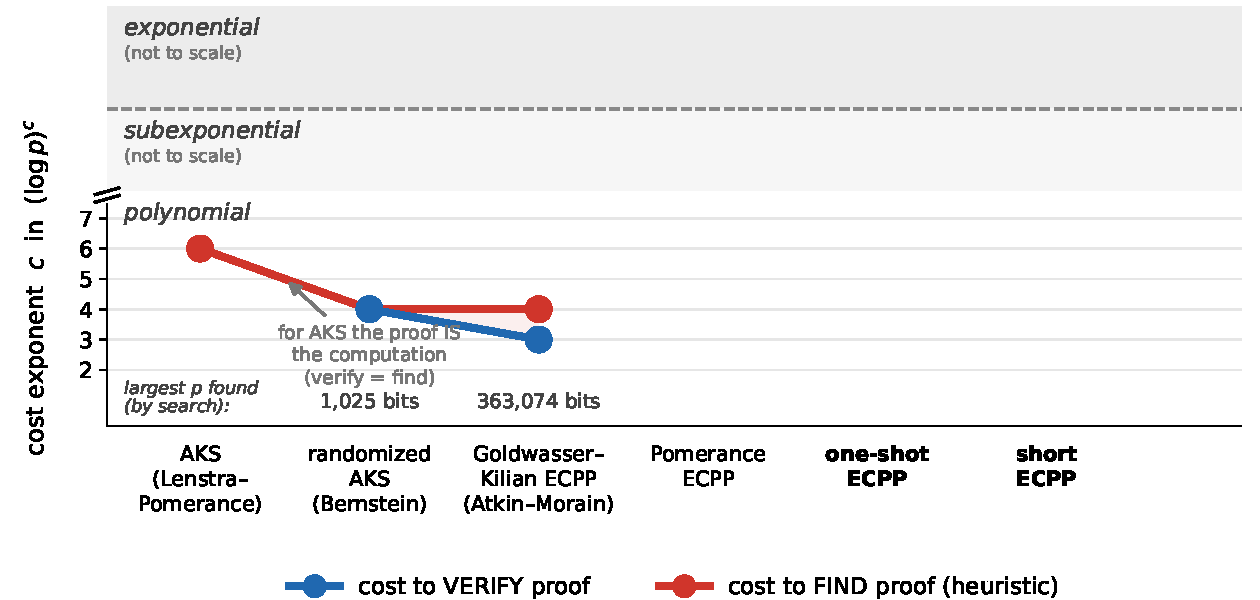
\includegraphics[width=0.95\paperwidth]{figs/gap-1.pdf}}%
\only<2>{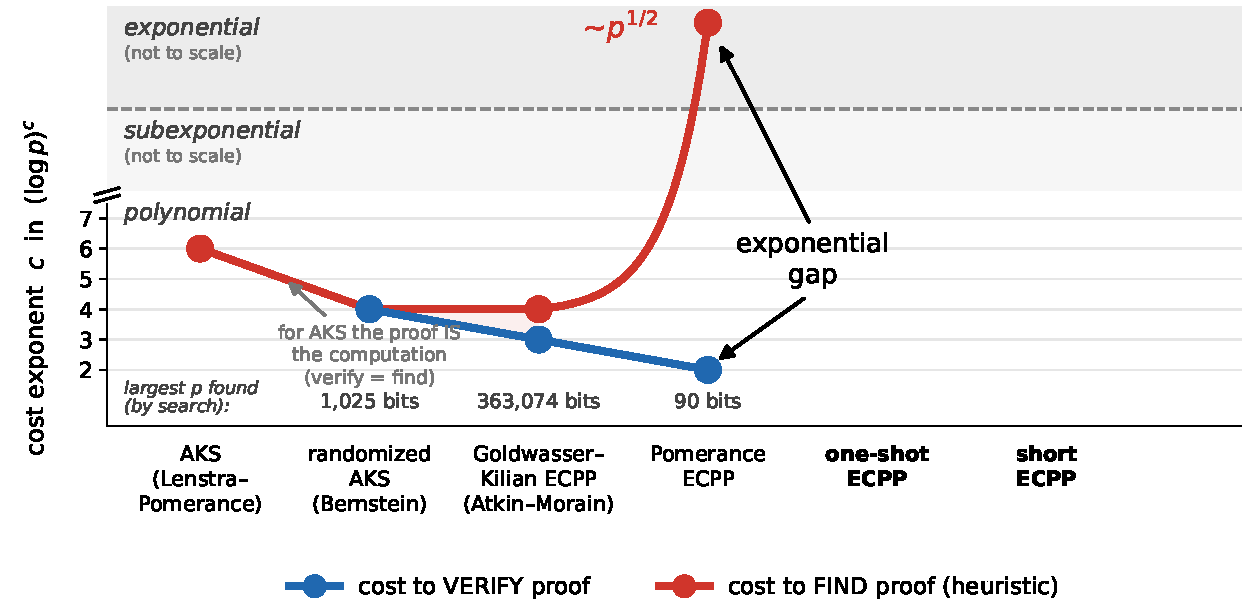
\includegraphics[width=0.95\paperwidth]{figs/gap-2.pdf}}}
\end{frame}

% ---------------------------------------------------------------------------
\begin{frame}{One lemma behind every elliptic certificate}
\begin{block}{Lemma (Goldwasser--Kilian 1986, Pomerance 1987)}
Let $p>3$ be odd and $L(p) = q+1+\lfloor 2\sqrt q\rfloor$ with $q = \lfloor\sqrt p\rfloor$.
If $x_0$ is the $x$-coordinate of a point of order \emph{exactly} $m > L(p)$ on
$By^2 = x^3 + Ax^2 + x$ \alert{modulo every prime $\ell \mid p$}, then $p$ is prime.
\end{block}
\textit{Proof.} Otherwise some prime $\ell\le\sqrt p$ divides $p$, and
$m \le \#E(\F_\ell) \le \ell + 1 + 2\sqrt\ell \le L(p) < m$. \hfill$\square$

\bigskip
The verifier runs the Montgomery $x$-only ladder (as in X25519) modulo $p$:
\begin{itemize}
\item $[m](x_0:1) = (X:0)$ with $\gcd(X,p) = 1$;
\item $[m/q](x_0:1) = (X:Z)$ with $\gcd(Z,p) = 1$ \ for each prime $q\mid m$.
\end{itemize}
No need to check that $x_0$ is on $E$: it is on $E$ or its twist, and the ladder serves both.

\bigskip
\alert{The verifier must know the factorization of $m$.}
Each format below is a rule for how $m$ may be built so that it can.
\end{frame}

% ---------------------------------------------------------------------------
\begin{frame}{Attacking the verifier}
\begin{itemize}
\item \textbf{The order of $P$ in $E(\Z/p\Z)$ is not enough.}
$p_0 = 4410667997551 = 2098153\cdot 2102167$ has a point of order exactly $8\cdot 525029 > L(p_0)$
in $E(\Z/p_0\Z)$: order $8$ modulo one factor and $525029$ modulo the other.\\
The gcd guards force order $m$ modulo \emph{every} $\ell\mid p$; a failed guard factors $p$
(ECM, run in reverse).
\medskip
\item \textbf{The fold attack.} One-shot certificates list the primes $q_i\in(n^2,n^4)$ of $m$.
Check them against $m$ rather than its $n^2$-rough part, and a repeated small prime $c$ can be
folded into a fake ``prime'' $cq$.
\medskip
\item \textbf{Cost attacks.} The verifier's cost bound must hold over \emph{all} certificates,
including malicious ones.  The August 2026 revision of short ECPP caps the smoothness bound and
the radical of each filler: $O(n^2\log n)$ bit operations, worst case, with no precomputation.
\end{itemize}
\end{frame}

% ---------------------------------------------------------------------------
\begin{frame}{Pomerance triples $(p, A, x_0)$: 2.5 Miller--Rabin rounds}
Let $k$ be least with $2^k > L(p)$.  Double $(x_0:1)$ $k$ times modulo $p$:
$\gcd(Z_{k-1},p) = 1$ and $Z_k \equiv 0$.
\begin{itemize}
\item \ver{Verify:} $5k \approx \tfrac52\log_2 p$ multiplications mod $p$, about
\ver{2.5 Miller--Rabin rounds}.
\item Exists for every prime $p>3$ (Pomerance 1987; descend the 2-isogeny volcano to make the
2-Sylow subgroup cyclic).
\item \find{Find:} $\#E$ must be one of the 2--4 multiples of $2^k$ in the Hasse interval, so
\find{$\Tt(\sqrt p)$ curves}.  Neither point counting nor CM helps.
Best test: one ladder projects $P$ into the 2-Sylow subgroup, then double with early abort.
\end{itemize}
\smallskip
\textbf{DANGER3 challenge} (BIRS, April 2026); every entry a human + AI collaboration:
\vspace{-0.3em}
\begin{center}\footnotesize
\begin{tabular}{@{}lrl@{}}
\toprule
$p$ & candidates & resources\\
\midrule
$10^{19}+51$ & $3.7\times 10^{9}$ & 400 s, multithreaded C (Apr 2026)\\
$10^{24}+7$ & $1.8\times 10^{10}$ & 6 h, laptop (Jun 2026)\\
$10^{26}+67$ & $1.4\times 10^{11}$ & 45 min, one RTX 6000 GPU (Jun 2026)\\
$10^{27}+103$ & $5.6\times 10^{12}$ & 52 min, 16 RTX 5090 GPUs (Aug 2026)\\
\bottomrule
\end{tabular}
\end{center}
\end{frame}

% ---------------------------------------------------------------------------
\begin{frame}{One-shot ECPP: relax $2^k$ to ``smooth''}
\textbf{Certificate} $(p, A, x_0, m, q_1,\dots,q_k)$ with $n = \lceil\log_2 p\rceil$:
$m$ is $n^4$-smooth, $L < m < rL$ ($r$ the least prime of $m$), and $q_1<\dots<q_k$ are the
primes of $m$ in $(n^2, n^4)$.
\begin{itemize}
\item \ver{Verify:} trial-divide $m$ by the primes below $n^2$ (remainder trees); what is left must be
exactly the $q_i$.  No primality tests needed: a composite in $(n^2, n^4)$ has no divisors
${>}\,n^2$.  \ver{$O(n^2(\log n)^2)$} bit operations.
\item \find{Find:} need the $n^4$-smooth part of $\#E$ to exceed $L\approx\sqrt p$.  By Dickman, this
happens with probability
\[
\rho(u/2)^{1+o(1)} = p^{-1/8+o(1)}, \qquad u = \frac{\ln p}{\ln n^4},
\]
so \find{$p^{1/8+o(1)}$} with random curves (SEA) and \find{$p^{1/4+o(1)}$} with the CM method.
The $o(1)$ is very negative: $1/\rho(u/2)\approx 200$ at 256 bits.
\item \emph{Restricted:} no list, $m$ must be $n^2$-smooth.  The exponent doubles to $1/4$:
${\approx}\,3\times10^7$ candidates at 256 bits.  A few hundred bits of listed primes
buy a factor of ${\sim}10^5$.
\end{itemize}
\end{frame}

% ---------------------------------------------------------------------------
\begin{frame}{Your favorite primes, certified}
\textbf{Curve25519:} \ $p = 2^{255}-19$, \ $n = 255$, \ $(n^2, n^4) = (65025,\ 4.2\times10^{9})$
\smallskip

{\footnotesize\ttfamily
A \ = 43723938096469358174465367825326655176206707707732910657972722225974945941308\\
x0 = 21311565618644507407816902738495363844983006752308652924886881573350137817662\\
m \ = 149 * 727 * 679409 * 770503 * 12519979 * 15032243 * 58136053 \quad\rmfamily(129 bits)\par}
\smallskip
Listed: the five primes after $727$.  Verified in 5\,ms (pure Python).
\medskip
\begin{center}\footnotesize
\begin{tabular}{@{}lp{0.62\textwidth}@{}}
\toprule
prime & how\\
\midrule
Curve25519, P-256, secp256k1 & CM search, 4--11\,s on 16 cores\\
BLS12-381 & CM search, 18\,s on 256 cores\\
P-384 & $p\equiv 3 \bmod 4$, so $y^2 = x^3+x$ has $p+1$ points; $p+1$ has a 197-bit $n^4$-smooth part\\
P-521 & $p+1 = 2^{521}$, so $y^2 = x^3+x$ gives a Pomerance triple with $m = 2^{261}$\\
\midrule
$10^{120}+79$ (generic, 399 bits) & CM search, minutes on 256 cores\\
\bottomrule
\end{tabular}
\end{center}
\end{frame}

% ---------------------------------------------------------------------------
\begin{frame}{Short ECPP: add recursion}
\textbf{Certificate} $(p_0;\ A_0, x_0, o_0;\ \dots;\ A_k, x_k, o_k)$; \
$n = \lceil\log_2 p_0\rceil$ fixed, \ $B = \lceil n^2/\log_2 n\rceil$.
\begin{itemize}
\item $o_i = m_i\cdot p_{i+1}$: \ $m_i$ is $B$-smooth with $\log_2\rad(m_i)\le\lceil n/\log_2 n\rceil$;
\ $p_{i+1}$ is $B$-rough with $B^2 < p_{i+1} < \sqrt{p_i}$.
\item $L(p_i) < o_i < r_iL(p_i)$; point of order exactly $o_i$ modulo every prime $\ell\mid p_i$.
\item Primality of $p_{i+1}$ is the next level's job.  Stop at $p_{k+1} < B^2$: $B$-rough and
below $B^2$ means $1$ or prime.
\end{itemize}
\medskip
\begin{center}
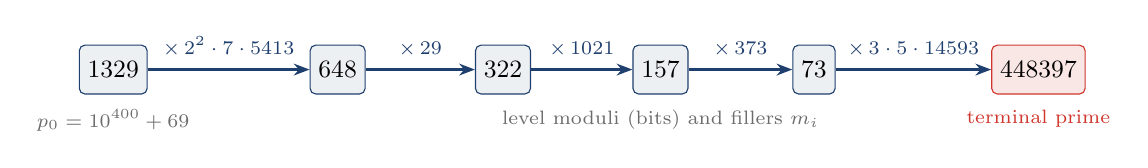
\begin{tikzpicture}[x=1cm,
  lev/.style={draw=dkblue,fill=dkblue!8,rounded corners=2pt,minimum height=0.62cm,
              inner sep=3pt,font=\small},
  arr/.style={-{Stealth[length=2mm]},thick,dkblue}]
\node[lev] (a) at (0,0)    {1329};
\node[lev] (b) at (2.85,0) {648};
\node[lev] (c) at (4.95,0) {322};
\node[lev] (d) at (6.95,0) {157};
\node[lev] (e) at (8.9,0)  {73};
\node[lev,fill=fred!12,draw=fred] (f) at (11.75,0) {448397};
\foreach \u/\v/\m in {a/b/{2^2\cdot7\cdot5413},b/c/{29},c/d/{1021},d/e/{373},e/f/{3\cdot5\cdot14593}}
  \draw[arr] (\u) -- node[above=1pt,font=\scriptsize] {$\times\,\m$} (\v);
\node[font=\scriptsize,color=grey,below=2pt of a] {$p_0 = 10^{400}+69$};
\node[font=\scriptsize,color=grey,below=2pt of d] {level moduli (bits) and fillers $m_i$};
\node[font=\scriptsize,color=fred,below=2pt of f] {terminal prime};
\end{tikzpicture}
\end{center}
\medskip
Bits at least halve: $O(\log n)$ levels, ${\lesssim}\,5n$ bits (6{,}328 here).
\ver{Verify: $O(n^2\log n)$} worst case, the order of a Pomerance triple.
\find{Find: subexponential.}
\end{frame}

% ---------------------------------------------------------------------------
\begin{frame}{Why finding is subexponential}
One level: find $E/\F_p$ with $\#E = S\cdot q$, $q$ prime ${\approx}\sqrt p$ (the next level).\\
The prover has to \emph{see} $q$: the rest of $\#E$ must peel off by ECM within a budget $y$.
\begin{itemize}
\item candidates needed: $1/\rho(u)$, \ $u = \ln\sqrt p\,/\ln y$ \hfill (Dickman)
\item cost per candidate: $L_y(1/2, \sqrt 2)$ \hfill (ECM)
\item balance with $\ln y = \gamma(\ln p)^{2/3}(\ln\ln p)^{1/3}$; the total is
$L_p\bigl(1/3,\ \tfrac{1}{6\gamma} + 2\sqrt{\gamma/3}\bigr)$, minimized at $\gamma = 12^{-1/3}$:
\end{itemize}
\[
\find{L_p\bigl(1/3,\ (3/2)^{1/3}\approx 1.14\bigr)},
\]
cheaper than factoring $p$ by the number field sieve, $L_p\bigl(1/3, (64/9)^{1/3}\approx 1.92\bigr)$,
which is also what a Pratt certificate costs.
\begin{itemize}
\item The same constant for both supplies of orders: random curves + SEA, or CM.  The CM
discriminant scan costs $L_p(1/3, 0.76)$ and never dominates.
\item Each level down shrinks the exponent by $2^{-1/3}$, so the top level dominates.
\end{itemize}
\vfill
\src{Heuristic: random-order model, Dickman, ECM.  The $o(1)$ converges like
$\ln\ln\ln p/\ln\ln p$, so constants are only indicative at feasible sizes.}
\end{frame}

% ---------------------------------------------------------------------------
\begin{frame}{Records, and the cost of checking them}
\begin{columns}[T]
\begin{column}{0.44\textwidth}
\textbf{Short ECPP records:} $\mathrm{nextprime}(10^c)$ for $c = 10, 20, \dots, 400$.
\begin{itemize}
\item Largest: $10^{400}+69$, 1329 bits, 5 levels, a 6{,}328-bit certificate.
\item $c = 320,\dots,400$: ${\approx}\,28{,}000$ core-hours, ${\approx}\,\$420$ of AWS spot
(192-core instances, six preemptions).
\item For comparison: one-shot reaches 399 bits; Pomerance triples reach 90 bits.
\end{itemize}
\end{column}
\begin{column}{0.54\textwidth}
\textbf{Cost to verify} (Python; same big-integer arithmetic as \texttt{pow}):
\smallskip

{\small
\begin{tabular}{@{}lrrr@{}}
\toprule
certificate & bits & time & MR rounds\\
\midrule
Pomerance triple & any & & 2.5\rlap{${}^{a}$}\\
one-shot, Curve25519 & 255 & 4.9\,ms & 85\rlap{${}^{b}$}\\
short, $10^{200}+357$ & 665 & 16\,ms & 21\\
short, $10^{310}+733$ & 1030 & 47\,ms & 27\\
short, $10^{400}+69$ & 1329 & 90\,ms & 27\\
\bottomrule
\end{tabular}

\scriptsize\color{grey}
${}^{a}$exact multiplication count \quad ${}^{b}$dominated by sieving primes below $n^2$}
\medskip

\alert{An unconditional proof costs less than OpenSSL's 64 Miller--Rabin rounds.}
\end{column}
\end{columns}
\end{frame}

% ---------------------------------------------------------------------------
\begin{frame}{Are short proofs hard to find?}
\vspace{-0.4em}
\makebox[\textwidth][c]{%
\only<1>{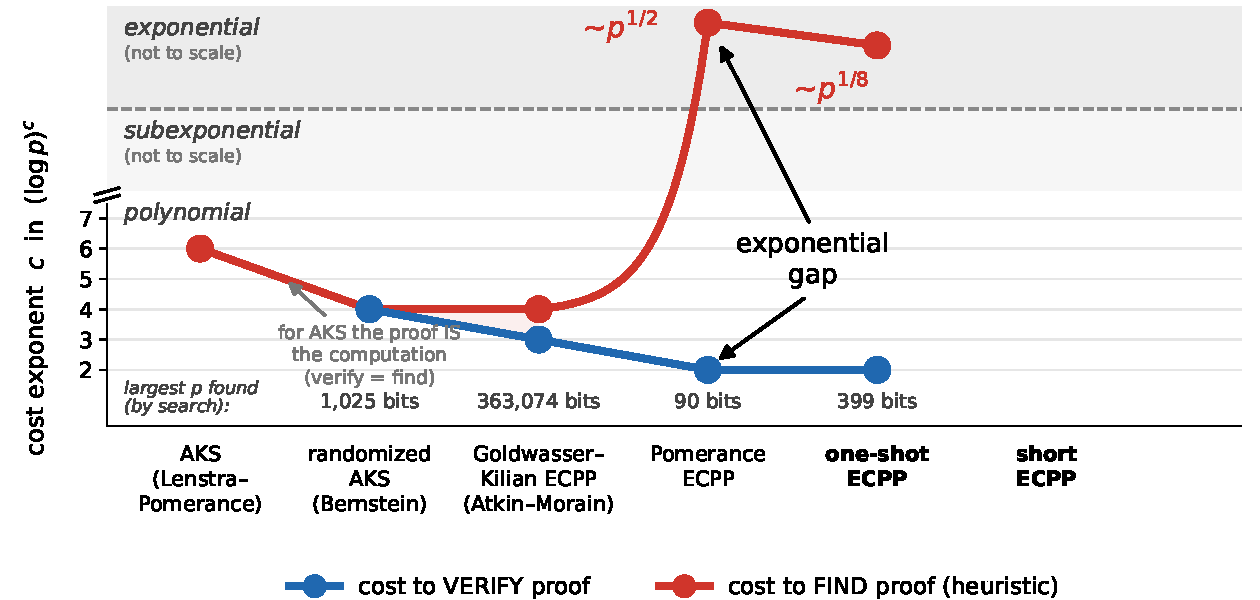
\includegraphics[width=0.95\paperwidth]{figs/gap-3.pdf}}%
\only<2>{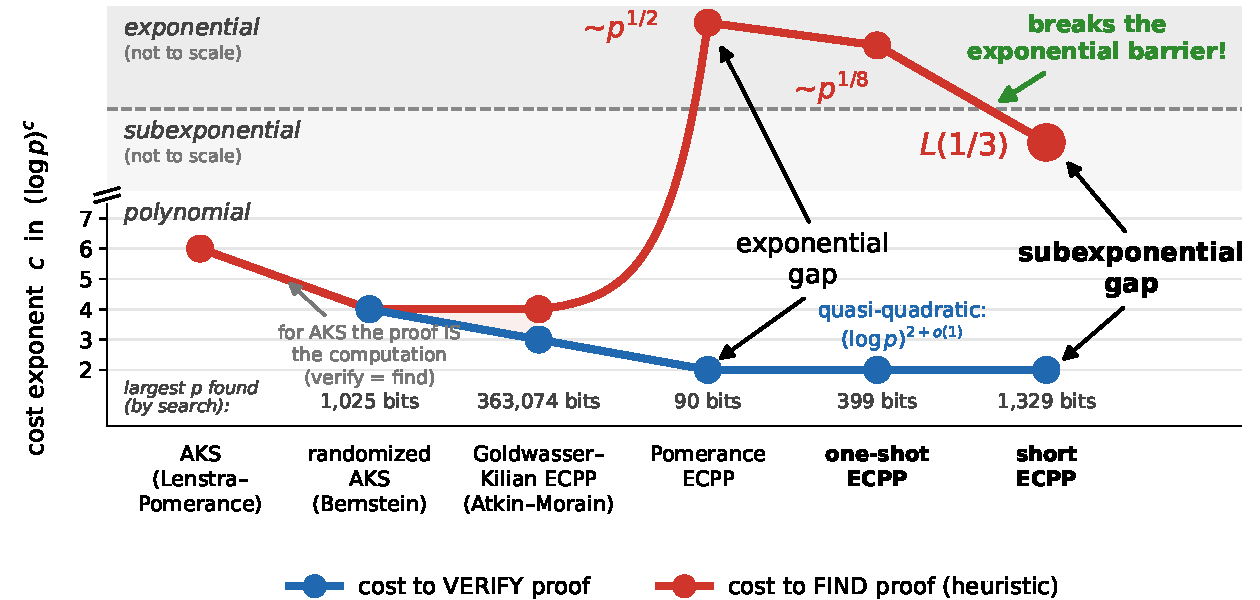
\includegraphics[width=0.95\paperwidth]{figs/gap-4.pdf}}}
\end{frame}

% ---------------------------------------------------------------------------
\begin{frame}{Open problems}
\begin{enumerate}
\item Beat \find{$\Tt(\sqrt p)$} for Pomerance triples, or explain why CM, isogenies, torsion
families and sieving cannot: ``$2^k \mid \#E$'' has no multiplicative structure to sieve on.
\medskip
\item One-shot via CM: close \find{$p^{1/4}$} vs.\ \find{$p^{1/8}$}.  This needs an
output-sensitive enumeration of $4p = t^2 + |D|v^2$ \emph{and} a root of $H_D \bmod p$ in
$h(D)^{1+o(1)}$ time.
\medskip
\item \alert{The find/verify trade-off.}  Is there a certificate with (even heuristic)
polynomial-time finding and $n^{2+o(1)}$ verification?
\begin{itemize}
\item AKS--Bernstein: \find{$(\log p)^{2+o(1)}$} to find, \ver{$(\log p)^{4+o(1)}$} to verify.
\item Short ECPP: \ver{$(\log p)^{2+o(1)}$} to verify, \find{$L(1/3)$} to find.
\end{itemize}
\medskip
\item Rigor: prove that a positive proportion of curves $E/\F_p$ have a $y$-smooth part of
$\#E$ exceeding $\sqrt p$.  Every finding bound here is heuristic.
\medskip
\item Is $\tfrac52\log_2 p$ multiplications optimal for general $p$?  Pomerance declined to
conjecture it.
\end{enumerate}
\end{frame}

% ---------------------------------------------------------------------------
\begin{frame}{Thank you}
\begin{itemize}
\item Survey:
\href{https://github.com/AndrewVSutherland2/OneShotFastECPP/blob/main/reports/ecpp-varieties/ecpp-varieties.pdf}
{\texttt{github.com/AndrewVSutherland2/OneShotFastECPP}}\\
\hspace*{1em}\texttt{reports/ecpp-varieties/ecpp-varieties.pdf}
\bigskip
\item Challenges (definitions, reference verifiers, leaderboards):
\begin{itemize}
\item \href{https://github.com/AndrewVSutherland/DANGER3}{\texttt{github.com/AndrewVSutherland/DANGER3}}
\item \href{https://github.com/AndrewVSutherland/OneShotPrimalityProofs}{\texttt{github.com/AndrewVSutherland/OneShotPrimalityProofs}}
\item \href{https://github.com/AndrewVSutherland/ShortPrimalityProofs}{\texttt{github.com/AndrewVSutherland/ShortPrimalityProofs}}
\end{itemize}
\bigskip
\item Certificates welcome.
\end{itemize}
\end{frame}

% ===========================================================================
\appendix
\begin{frame}{Backup: the certificate families}
\centering\footnotesize
\setlength{\tabcolsep}{4pt}
\resizebox{\textwidth}{!}{%
\begin{tabular}{@{}lllll@{}}
\toprule
certificate & size (bits) & verify (bit ops) & find (heuristic) & exists for\\
\midrule
Pratt & $O(n^2)$ & $O(n^3\log n)$ & $L_p(1/3, 1.923)$ (NFS) & all $p$\\
AKS--Bernstein & $n^{1+o(1)}$ & $(\log p)^{4+o(1)}$ & $(\log p)^{2+o(1)}$ randomized & all $p$\\
Pomerance triple & ${\approx}\,2n$ & $O(n^2\log n)$ & $\Tt(\sqrt p)$ & all $p>3$\\
restricted one-shot & ${\approx}\,2.5n$ & $O(n^2(\log n)^2)$ & $p^{1/4+o(1)}$ SEA;\ $p^{1/2+o(1)}$ CM & all $p>3$\\
one-shot ($n^4$-smooth) & ${\approx}\,2.5n$--$3n$ & $O(n^2(\log n)^2)$ & $p^{1/8+o(1)}$ SEA;\ $p^{1/4+o(1)}$ CM & all $p>3$\\
short ECPP & ${\lesssim}\,5n$ & $O(n^2\log n)$ & $L_p(1/3, 1.14)$, SEA \& CM & all $p\ge5$\\
classical ECPP & $\Theta(n^2/\log n)$ & $O(n^3)$ & $(\log p)^{6+o(1)}$ SEA;\ $(\log p)^{4+\epsilon}$ CM & all $p$ (heur.)\\
\bottomrule
\end{tabular}}

\bigskip
\raggedright\small
Existence for every $p$ passes from Pomerance's theorem to every format containing his triples.
\end{frame}

\begin{frame}{Backup: two engines for candidate orders}
\begin{itemize}
\item \textbf{SEA:} pick a random curve and count its points.  Polynomial cost per candidate,
flat forever (stock PARI: 7--14 core-seconds at 384--448 bits); both twists come free.
\item \textbf{CM:} pick $D$ with $4p = t^2 + |D|v^2$; orders $p+1\pm t$ known before any curve
exists.  ${\sim}10^7$ discriminants/s, but $|D|\le B$ yields only ${\approx}\,0.45\sqrt B$ usable
orders, so $K$ candidates cost $K^2$; the winner needs a class polynomial of degree
${\approx}\sqrt{|D|}$ (largest so far: $h = 35{,}085$).
\end{itemize}
\medskip
\textbf{One-shot race}, same primes, 192-core machines:
\begin{center}\small
\begin{tabular}{@{}rrrrr@{}}
\toprule
bits & $1/\rho(u/2)$ & CM wall & SEA wall & core-s/candidate (SEA vs CM)\\
\midrule
256 & $2.0\times10^2$ & 4.1 s & 68 s & ---\\
384 & $1.6\times10^4$ & 2{,}306 s & 615 s & 7.2 vs 3.5\\
416 & $4.8\times10^4$ & 1{,}774 s & 2{,}805 s & 10.1 vs 2.2\\
448 & $1.6\times10^5$ & 7{,}182 s & stopped at 20{,}035 s & 13.7 vs 4.5\\
\bottomrule
\end{tabular}
\end{center}
Crossover extrapolates to ${\approx}\,480$--$512$ bits for one-shot and ${\approx}\,2000$ bits for
short ECPP.
\end{frame}

\begin{frame}{Backup: restricted one-shot ($n^2$-smooth $m$, no list)}
\centering\small
\begin{tabular}{@{}lrrl@{}}
\toprule
bits & $u/2$ & $1/\rho(u/2)$ & SEA cost\\
\midrule
67 ($10^{20}$) & 2.74 & 12 & seconds, one core\\
133 ($10^{40}$) & 4.71 & $1.3\times10^3$ & minutes, one core\\
167 ($10^{50}$) & 5.62 & $1.7\times10^4$ & ${\approx}\,1$--$2$ core-hours\\
200 ($10^{60}$) & 6.52 & $2.5\times10^5$ & ${\approx}\,10^2$--$10^3$ core-hours\\
256 & 8.00 & $3.1\times10^7$ & ${\approx}\,5$--$10$ core-years\\
384 & 11.18 & ${\approx}\,3\times10^{12}$ & out of reach\\
\bottomrule
\end{tabular}

\bigskip
\raggedright
First generic certificates: $10^{20}+39$, $10^{30}+57$, $10^{40}+121$, $10^{50}+151$.  E.g.\
$m = 2\cdot3\cdot7\cdot29\cdot37\cdot211\cdot337\cdot347\cdot449\cdot467\cdot3527\cdot12613$ for
$10^{50}+151$.\\[4pt]
Unrestricted one-shot at 256 bits: 4 seconds.
\end{frame}

\begin{frame}{Backup: the AKS--Bernstein certificate}
\begin{itemize}
\item Tuple $(d, e, c, c_-, f, r, S)$: $f$ of degree $d$ over $\Z/p\Z$, $e \mid p^d - 1$; validity
forces $p$ to be a prime power (Berrizbeitia, Cheng, Mih\u{a}ilescu--Avanzi, Bernstein 2007).
\item Every prime has one of size $n^{1+o(1)}$, \find{found in expected $(\log p)^{2+o(1)}$},
\ver{verified in $(\log p)^{4+o(1)}$}.  Example: $(1, 57449, 28724, 16826, y, 2, \{1\})$ for
$2^{1024}+643$.
\item The asymmetry is inverted: a Las Vegas verifier gains nothing from the certificate, since it
can regenerate one itself in less time than the check takes.  What it buys is determinism.
\item Verification is stuck at quartic: soundness forces $e = \widetilde\Omega(\log^2 p)$, a ring
of $(\log p)^{3+o(1)}$ bits.
\end{itemize}
\end{frame}

\begin{frame}{Backup: descent chains with ratio $b$}
\begin{itemize}
\item Chain of certificates with $q \le p^b$ at each step, $b\in(\tfrac12, 1)$, order $c\cdot q$
with no minimality required.
\item Size $O(n)/(1-b)$; \ver{verify $O(n^2\log n)/(1-b^2)$}; \find{find
$L_p\bigl(1/3, (3(1-b))^{1/3}\bigr)$}.
\item With $b = 0.85$ on a 16-core desktop: $2^{255}-19$ and $10^{100}+267$ in 3.7\,s each
(one-shot: ${\approx}\,15$\,s and 7.9\,min), and
\begin{center}\small
\begin{tabular}{@{}lrrr@{}}
\toprule
$p$ & find & steps & verify\\
\midrule
1024 bits & 128 s & 9 & 0.41 s\\
2048 bits & 5.2 h & 12 & 2.65 s\\
\bottomrule
\end{tabular}
\end{center}
\item $b = \tfrac12$ with minimal orders is short ECPP; $b\to1$ heads toward classical ECPP
(qualitatively).
\end{itemize}
\end{frame}

\end{document}
